\documentclass{article}
\usepackage[utf8]{inputenc}
\usepackage[T2A]{fontenc}
\usepackage[russian,english]{babel}
\usepackage{amssymb}
\usepackage{amsmath}\usepackage[pdftex]{graphicx}
\usepackage{fancyhdr} 
\usepackage[left=3cm,right=3cm,
top=2.5cm,bottom=2.5cm,bindingoffset=0cm]{geometry}
\begin{document}
\selectlanguage{russian}
\fancyhead[CO]{ОБРАТНАЯ ФУНКЦИЯ}
\pagestyle{fancy}
В.Г.Болтянский
\\(Москва)
\\ОБРАТНАЯ ФУНКЦИЯ
\par Функция -- одно из важнейших понятий современной математики. Несмотря на это, основные определения и терминология, связанные с функиями, до сих пор не являются устоявшимися и унифицированными. Ученые, работающие в разных областях математики, применяют разную терминологию; например, в анализе чаще используется термин <<функция>>, в топологии -- <<отображение>>, в функциональном анализе -- <<функционал>>, <<оператор>> и т.д. Существуют и разные тенденции в понимании смысла функции. Так, одна тенденция (идущая, по-видимому, от книг американского тополога Келли) состоит в том, что рассматриваются только сюръективные отображения, т.е. отображения одного множества на другое. Она принята сейчас в школьных учебниках алгебры. Одна из основных отличительных черт этой тенденции состоит в том, что если каждому элементу $x$ множества $A$ поставлен в соответствие некоторый элемент $f(x)\in B$, причем не все элементы множества $B$ являются образами элементов из $A$, то можно выбросить из $B$ <<лишние>> элементы (в примере на рис.1 они обведены штриховой рамкой), благодаря чему f станет отображением множества $A$  на некоторое множество $B'\subset B$. Считая, что каждый раз <<лишние>> элементы автоматически отбрасываются, мы и приходим к рассмотрению только сюръективных отображений.
\\
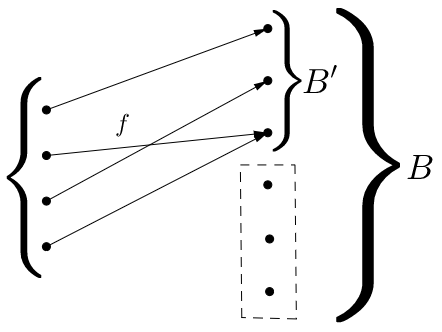
\includegraphics[scale=0.4]{obrfunc.png}(рис.1)
\par Другая тенденция (назовем ее условно <<тенденцией Бурбаки>>) состоит в том, что $f\colon A\to B$ и $f\colon A \to B'$ -- это разные отображения (в связи с чем второе из них правильнее обозначать не $f$, а другой буквой). Этой тенденции придерживается большая часть современных математиков. Достаточно сказать, что вся алгебраическая топология и другие разделы математики (связанные с рассмотрением так называемых категорий и функторов) немыслимы без такого различения. В связи с этим рассматриваются не только сюръективные отображения, но и отображения, не являющиеся сюръективными (отображения одного множества в другое).
\par Приведу два примера, иллюстрирующие большую гибкость и удобство <<тенденции Бурбаки>> по сравнению с <<тенденцией Келли>>.
\par Формула $y=x^6+2x^2-11x$ задает некоторую числовую функцию, областью определения которой служит вся числовая прямая $\mathbb{R}$. Однако множество значений этой функции есть какой-то луч $[a;+\infty]$, который мы не знаем (для нахождения минимума выражения $x^6+2x^2-11x$ нужно было найти корень производной, т.е. решить уравнение пятой степени). Вместе с тем ясно, что эта функция ставит в соответствие любому числу $x\in \mathbb{R}$ некоторое число (также принадлежащее $\mathbb{R}$), т.е представляет собой отображение $\mathbb{R}$ снова в множество $\mathbb{R}$. Вряд ли выбрасывание <<лишних>> элементов, т.е. замена области значений $\mathbb{R}$ множеством значений (т.е. лучом, который мы не знаем), способствует достижению у школьников яности понимания (ведь речь идет о такой простой функции, как многочлен!).
\par В качестве второго примера отметим, что плоскость $P$ является односвязной фигурой: тождественные отображение $e:K\to P$ любой замкнутой линии $K$ в плоскость $P$ может быть непрерывно продеформировано (рис.2)
\\
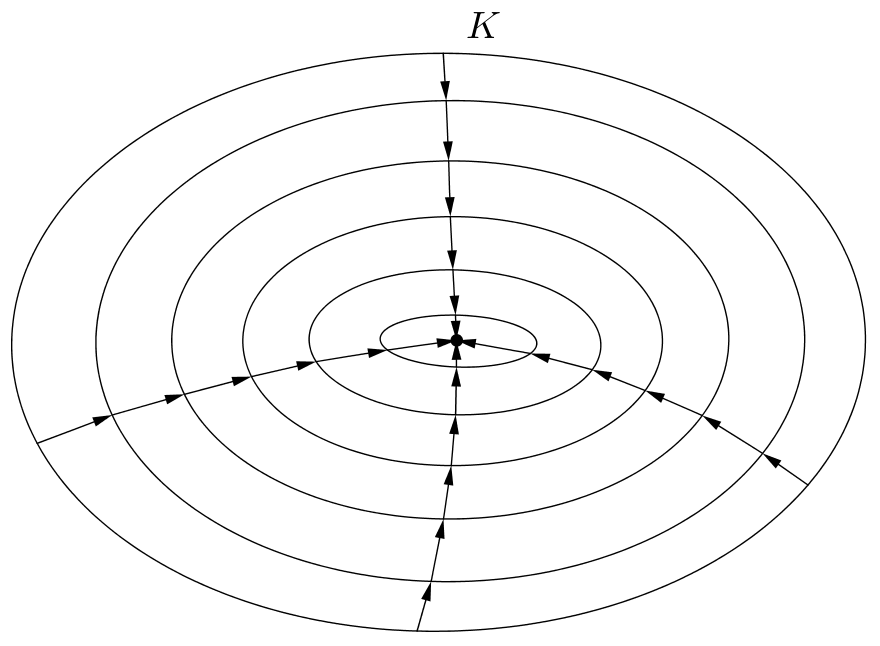
\includegraphics[scale=0.2]{k.png}(рис.1)
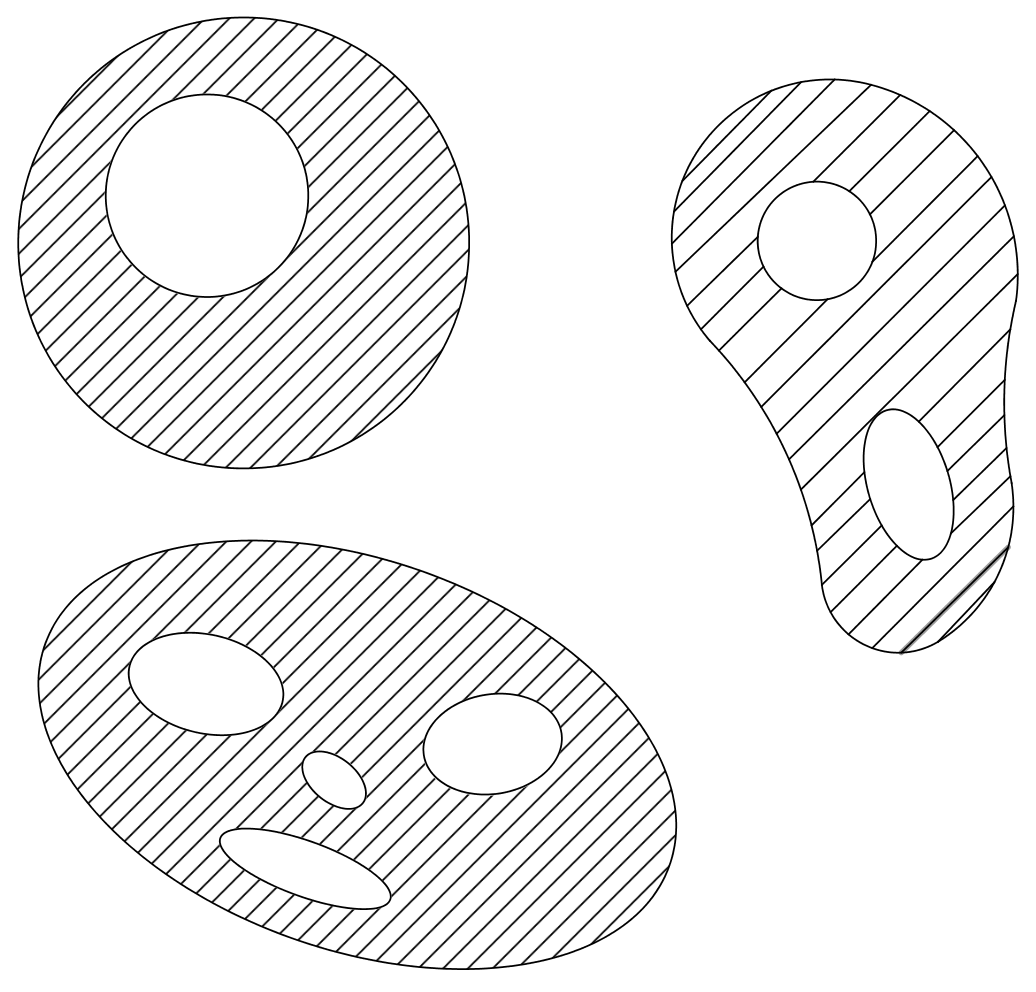
\includegraphics[scale=0.2]{faces.png}(рис.2)
\\в отображение всей линии $K$ в одну точку, или, как говорят для краткости, отображение $e$ стягиваемо в точку. Однако тождественное отображение $e:K\to K$ линии $K$ на себя нельзя стянуть в точку (т.е.перемещая, деформируя линию по самой себе, а не по плоскости, мы не сможем осуществить стягивание ее в точку). Это связано как раз с наличием <<лишних>> элементов у отображения $e:K\to P$. В отличие от плоскости кольцо и другие фигуры, изображенные на рис.3, неодносвязны. Понятие односвязаности является одним из основополагающих в алгебраической топологии, в теории функций комплексного переменного, в анализе. Выбрасывание <<лишних>> элементов зачеркнуло бы эти области математики!
\par Было бы неправильным ограничивать кругозор учителя, считая, что если тенденции и определения не соответствуют сегодняшним учебникам, то они <<не верны>>.
\par В предлагаемой статье дается подход к понятию обратной функции (и связанным с ней вопросам школьного курса) с точки зрения <<тенденции Бурбаки>>. Учитель легко разберется, где определения, принятые в статье, соответствуют принятым сейчас в учебниках алгебры, а где расходятся с ними.
\\\textbf{1.Общие свойства обратных отображений}
\par Пусть $f$ -- некоторое отображение множества $A$ в множество $B$ (для краткости пишут $f\colon A\to B$). Это означает, что каждому элементу $x_0\in A$ поставлен с соответствие какой-то элемент множества $B$, обозначаемый через $f(x_0)$ и называемый образом элемента $x_0$ при отображении $f$. Множество A называется областью определения отображения $f$, а $B$ -- множеством значений этого отображения.
\par Пусть $f\colon A\to B$. Возьмем произвольный элемент $y_0\in B$. Множество всех корней уравнения\footnote[1]{Несмотря на то что речь идет о произвольном отображении $f\colon A\to B$ (не заданном с помощью аналитического выражения), имеет смысл говорить о решении <<уравнения>>, т.е. о нахождении всех тех $x\in A$, при которых соотношение $f(x)=y_0$ превращается в истинное высказывание.} $f(x)=y_0$ называется прообразом элемента $y_0$ и обозначается через $f^{-1}(y_0)$. Иначе говоря, элемент $x_0\in A$ в том и только в том случае принадлежит множеству $f^{-1}(y_0)$, если $f(x_0)=y_0$.
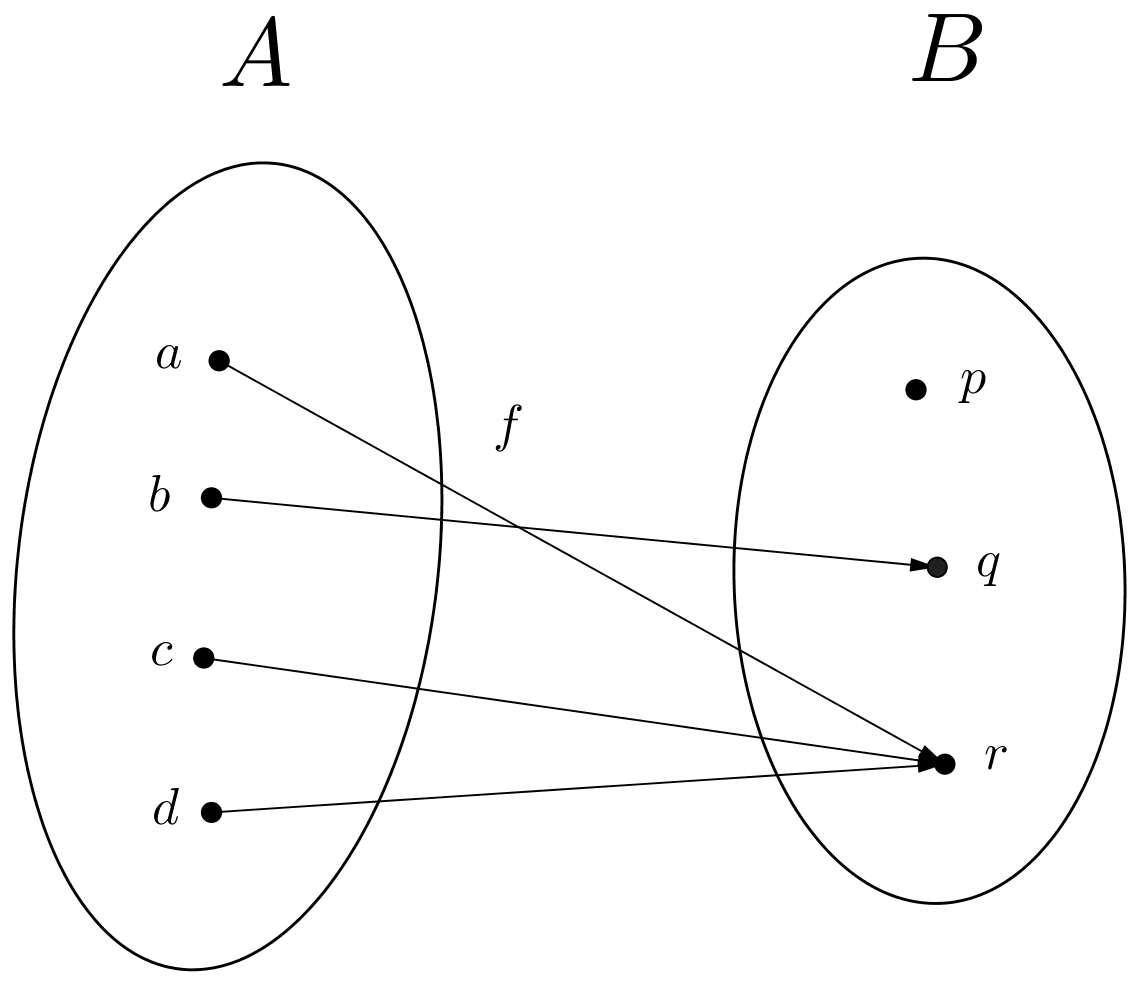
\includegraphics[scale=0.25]{ovals.png}(рис.4)
\par Прообраз $f^{-1}(x)$ может быть пустым множеством, а может состоять из одного, двух или большего (даже бесконечного) числа элементов. Так, для отображения $f\colon A\to B$, показанного на рис.4, прообразы элементов будут следующими:
$$f^{-1}(p)=\varnothing, f^{-1}(q)=\{b\}$$
$$f^{-1}(r)=\{a; c; d\}$$
\par Если для любого элемента $y_0\in B$ его прообраз $f^{-1}(y_0)$ состоит ровно из одного элемента, то отображение $f\colon A\to B$ называется биективным (или взаимно-однозначным). В случае биективного отображения $f\colon A\to B$ принято записывать прообразы без фигурных скобок: если $f(x_0)=y_0$, то пишут
$$f^{-1}(y_0)=x_0.$$
Этим определяется некоторое отображение $B\to A$, которое называется обратным к отображению $f$ и обозначается через $f^{-1}$
\par Обратное отображение как бы возвращает элементы на свои места. Если отображение $f$ переводит элемент $x_0 \in A$ в элемент $y_0\in B$, то отображение $f^{-1}$ переводит $y_0$ обратно в $x_0$ (этим и объясняется название обратное отображение). Ясно, что обратное отображение $f^{-1}$ также является биективным, причем обратным к $f^{-1}$ является исходное отображение $f$, т.е. $(f^{-1})^{-1}=f$. На этом основании говорят, что отображения $f$ и $f^{-1}$ являются взаимно-обратными.
\par Из сказанного выше непосредственно следует, что при переходе к обратному отображению область определения и область значений меняются местами, т.е. если $f\colon A\to B$ - произвольное биективное отображение, то обратное отображение $f^{-1}$ определено на множестве $B$ и имеет область значений $A$,
$$f^{-1}:B\to A.$$
\par Легко видеть, что композиция $f^{-1}\circ f$, т.е. результат последовательно выполнения сначала отображения $f$, а затем отображения $f^{-1}$ представляет собой тождественное отображение множества $A$. В самом деле, если $f(x_0)=y_0$, то
$$(f^{-1}\circ f)(x_0)=f^{-1}(f(x_0))=f^{-1}(y_0)=x_0$$
Следовательно, отображение $f^{-1}\circ f$ переводит элемент $x_0$ в себя. Так как это справедливо для любого элемента $x_0 \in A$, то $f^{-1}\circ f$ -- тождественное отображение. Точно так же композиция $f^{-1}\circ f$ (сначала выполняется $f^{-1}$, затем $f$) есть тождественное отображение множества $B$. Условившись обозначать тождественное отображение символом $id$ (от английского identity - тождество), можем написать
\begin{equation}\label{E1}
f^{-1}\circ f=id,f\circ f^{-1}=id
\end{equation}
\\Сформулируем доказанную теорему.
\par \textbf{Теорема  1.} Пусть $f\colon A\to B$ -- произвольное биективное отображение, а $f^{-1}\colon B\to A$ -- обратное к нему отображение. Тогда верны равенства \eqref{E1}.
\par Важно отметить, что теорема, обратная теореме 1, также верна.
\par \textbf{Теорема  2.} Пусть $f\colon A\to B$ и $g\colon B\to A$ -- некоторые отображения. Если справедливы соотношения 
\begin{equation}\label{E2}
g\circ f=id, f\circ g=id,
\end{equation}
то оба отображения $f,g$ биективны и являются взаимно-обратными.
\par \textbf{Доказательство.} Прежде всего установим биективность отображения $f$. Пусть $y_0$ -- произвольный элемент множества $B$.  Положим $x_0=g(y_0)$. Тогда $f(x_0)=f(g(y_0))=(f\circ g)(y_0)$ (поскольку $f\circ g = id$). Итак,
$$x_0\in f^{-1}(y_0).$$
\par Допустим, что существует еще один элемент 
$$x_1\in f^{-1}(y_0)$$
т.е. элемент $x_1\in A$, удовлетворяющий условию $f(x_1)=y_0$. Применяя отображение $g$, находим $g(f(x_1))=g(y_0)=x_0$, т.е. $(g\circ f)(x_1)=x_0$. Но так как $g\circ f=id,$ то $(g\circ f)(x_1)=x_1$ Следовательно, $x_0=x_1$.
\par Таким образом доказано, что дли любого $у_0\in В$ прообраз $f^{-1}(y_0)$ состоит из одного элемента. Это, по определению, означает, что отображение $f$ биективно.
\par Полученное в процессе доказательства соотношение $f(x_0)=y_0$ означает, что $f^{-1}(y_0)=x_0$. Но первоначально мы определили элемент $x_0$ равенством $x_0=g(y_0)$. Таким образом, $g(y_0)=f^{-1}(y_0)$. Поскольку это справедливо для любого элемемта $y_0\in B$, отображение $g$ совпадает с $f^{-1}$.
\par \textbf{Пример 1.} Пусть $A$ — плоскость, $B$ — некоторая содержащаяся в этой плоскости прямая. Через $f$ обозначим ортогональное проектирование плоскости $А$ на прямую $В$. Далее через $g\colon B\to A$ обозначим отображение, которое произвольной точке $М\in В$ ставит в соответствие ту же самую точку (но уже рассматриваемую как элемент множества $A$). Ясно, что если $N\in В$, то верны равенства $f(N)=N$, $g(N)=N$, и потому $f\circ g=id$, т. е. выполнено второе из соотношений \eqref{E2}. Первое же из этих соотношений не выполнено:	легко видеть, что $g\circ f=f$. Поэтому отображения $f$ и $g$ не являются взаимно-обратными. Этот пример показывает, что выполнения только одного из равенств \eqref{E2} недостаточно для справедливости заключения теоремы 2.
\par Пусть $f\colon A\to B$ -- произвольное отображение. Обозначим через $E(f)$ множество всех тех элементов $у_0\in B$, для которых прообраз $f^{-1}(y_0)$ является непустым множеством. Множество $E(f)$ называется образом (или множеством значений) отображения $f$.
\par Если отображение $f\colon A\to B$ удовлетворяет условию $B=E(f)$, то оно называется сюръективным отображением (или отображением множества $А$ на множество $B$).
\par Далее, отображение $f\colon A\to B$ называется инъективным, если для любого элемента $y_0\in B$ прообраз $f^{-1}(y_0)$ либо является пустым множеством, либо состоит ровно иэ одного элемента. Легко видеть, что отображение $f\colon A\to B$ в том и только в том случае является биективным, если оно сюръективно и инъективно одновременно. В самом деле, сюръективность означает, что для любого $y_0\in B$ прообраз $f^{-1}(y_0)$ является непустым множеством, и потому (в силу инъективности) он состоит ровно из одного элемента.
\\\textbf{2. Числовые функции}
\par Числовой функцией условимся называть всякое сюръективное отображение $f\colon A\to B$, где $A\subset\mathbb{R},B\subset \mathbb{R}$.
\par Наиболее часто употребляемым способом задания числовой функции является запись ее равенством, в левой части которого стоит $y$, а в правой — некоторое выражение, содержащее переменную $х$. Например,
$$y=x^2,\quad y=\sqrt{x-1}+lg(x^2-5)$$
и т. д. Когда говорят, что такая запись определяет некоторую числовую функцию $f$, то имеют в виду следующие соглашения:
\par 1.	Областью определения $А$ функции $f$ является множество всех тех действительных чисел, при подстановке которых вместо $x$ выполнимы (в области действительных чисел) все действия, указанные в рассматриваемом выражении.
\par 2. Если $x_0\in A$, то за $f(x_0)$ принимается значение стоящего в правой части выражения при $х=х_0$.
\par 3.	Функция $f$ сюръективна, т. е. областью ее значений является множество всех чисел вида $f(x_0)$, где $х\in A$,
\par Если $F(x)$ — некоторое выражение с переменной $х$, то для краткости вместо <<числовая функция, определенная равенством $y=F(x)$>> говорят просто <<функция $y=F(x)$>>. Именно в этом смысле употребляются привычные для школьного обихода обороты <<функция $y=x^2$>>, <<функция $y=\sin x$>> и т. п.
\par Заметим, что часто числовая функция задается несколькими различными формулами, рассматриваемыми на непересекающихся промежутках. Например, функция $y=|x|$ определяется следующим образом:
$$y=
\begin{cases}
x&\text{при} x\ge 0\\
-x&\text{при} x<0
\end{cases}
$$
В таких записях традиционно используется фигурная скобка, означающая, что правая часть рассматривается как единое выражение.
\par Пусть $F(x)$ — некоторое выражение с переменной $x$. Обозначим через $А$ область определения функции
\begin{equation}\label{E3}
y=F(x),
\end{equation}
а через $B$ — множество ее значений. Предположим, что соотношение \eqref{E3}, рассматриваемое как уравнение относительно $x$, имеет для любого $y\in B$ ровно один корень, который можно явно найти в виде выражения $G(y)$. Тогда справедлива следующая теорема.
\par\textbf{Теорема 3.}  Функция $y=G(x)$ является обратной для функции $y=F(x)$.
\par \textbf{Доказательство.} Для удобства обозначим функцию $y=F(x)$ через $f$, а функцию $y=G(x)$ — через $g$. Если $x_0\in A$, то число $y_0=F(x_0)$ является образом точки $x_0$ при отображении f, т. е. $y_0=f(x_0).$ Кроме того, равенство $y_0=F(x_0)$ означает, что $x_0$ есть корень уравнения \eqref{E3} при $y=y_0$, иначе говоря, $x_0=G(y_0).$ Следовательно, $x_0$ есть образ точки $y_0$ при отображении g, $x_0=g(y_0).$ Таким образом,
$$(g\circ f)(x_0)=g(f(x_0))=g(y_0)=x_0$$
и $f\circ g$ есть тождественное отображение множества $B$.
\par Пусть теперь $y_1\in B$. Тогда уравнение \eqref{E3} имеет при $y=y_1$ единственный корень $x_1=G(y_1)$. Отсюда можно сделать 2 вывода: 1) $x_1=g(y_1)$, 2) $y_1=F(x_1)$, т.е. $y_1=f(x_1)$. Таким образом,
$$(g\circ f)(y_1)=f(g(y_1))=f(x_1)=y_1$$
и $f\circ g$ есть тождественное отображение множества $B$.
\par Мы видим, что $g\circ f=id$, $f\circ g=id$, и потому, согласно теореме 2, $g=f^{-1}$.
\par \textbf{Замечание.} Соотношение \eqref{E3}, рассматриваемое как уравнение относительно $x$, имеет корень только при $y\in B$ (так как $B = E(f)$). Следовательно, если установлено, что уравнение \eqref{E3} имеет при любом $y\in \mathbb{R}$ не более одного корня, то это означает, что при $y\notin B$ оно корней не имеет, а при $y\in B$ имеет ровно один корень. Таким образом, мы получаем следующее практическое правило для нахождения функции $y=G(x)$, обратной для функции $y=F(x).$
\par Решить уравнение \eqref{E3} относительно $x$ (убедившись в процессе решения, что это уравнение имеет не более одного корня) и записать этот корень в виде $x=G(y)$. где $G(y)$ — некоторое выражение, содержащее переменную $y$. Если это удастся, то надо затем поменять местами $x$ и $y$, т. е. написать $y=G(x)$.
\par Это практическое правило удобно тем, что не требует предварительно находить область определения и множество значений функции \eqref{E3}: при правильном решении уравнения \eqref{E3} получаемое выражение $G(y)$ имеет в качестве своей области определения множество $B$ (т е. множество значений функции $y=F(x)$).
\par\textbf{Пример 2.} Найти функцию, обратную следующей:
\begin{equation}\label{E4}
y=\frac{2x-1}{x-2}
\end{equation}
\par\textbf{Решение.} Рассматривая соотношение \eqref{E4} как уравнение относительно $x$, находим (при $y\ne 2$) единственный корень
$$x=\frac{2y-1}{y-2}$$
\end{document}
